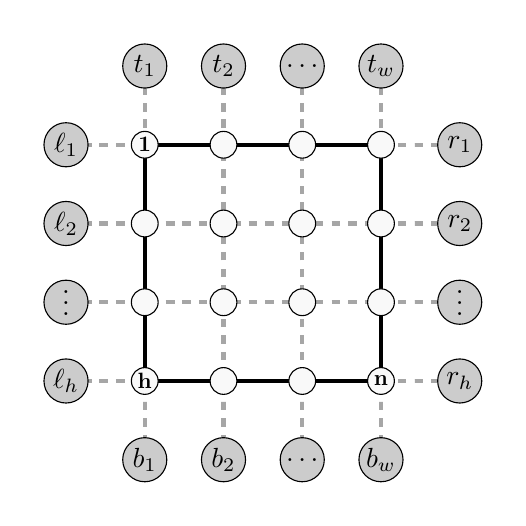
\begin{tikzpicture}
\foreach \x in {0,...,3}{
  \draw[dashed, line width=1.5pt, gray!70] (\x,-1) to[out=90,in=-90] (\x,4);
  \draw[dashed, line width=1.5pt, gray!70] (-1,\x) to[out=0,in=180] (4,\x);
}
\draw[line width=1.5pt] (0,0) -- (0,3);
\draw[line width=1.5pt] (0,0) -- (3,0);
\draw[line width=1.5pt] (0,3) -- (3,3);
\draw[line width=1.5pt] (3,0) -- (3,3);

\foreach \x in {0,...,3} 
	\foreach \y in {0,...,3}
   		\draw[fill = gray!5] (\x,\y) circle (1.7mm); 
   		
\foreach \x in {0,...,3} {
  \draw[fill = gray!40] (\x,-1) circle (2.8mm); 
  \draw[fill = gray!40] (-1,\x) circle (2.8mm); 
  \draw[fill = gray!40] (\x,4) circle (2.8mm); 
  \draw[fill = gray!40] (4,\x) circle (2.8mm); 
}
\draw[white] (-1.2,-1.2) circle (2.8mm);
\draw[white] (4.2,4.2) circle (2.8mm); 
\draw[white] (-1.2,4.2) circle (2.8mm); 
\draw[white] (4.2,-1.2) circle (2.8mm); 
   
   		
\node[scale = 0.8] at (0,3) {$\mathbf{1}$};
\node[scale = 0.8, above=-7pt] at (0,0) {$\mathbf{h}$};
\node[scale = 0.8] at (3,0) {$\mathbf{n}$};
\node at (0,4) {$t_1$};
\node at (1,4) {$t_2$};
\node at (2,4) {$\ldots$};
\node at (3,4) {$t_w$};

\node at (0,-1) {$b_1$};
\node at (1,-1) {$b_2$};
\node at (2,-1) {$\ldots$};
\node at (3,-1) {$b_w$};

\node at (4,3) {$r_1$};
\node at (4,2) {$r_2$};
\node[above=-8.5pt] at (4,1) {$\vdots$};
\node at (4,0) {$r_h$};

\node at (-1,3) {$\ell_1$};
\node at (-1,2) {$\ell_2$};
\node[above=-8.5pt] at (-1,1) {$\vdots$};
\node at (-1,0) {$\ell_h$};
\end{tikzpicture}